\section{Conclusion}\label{sec:conclusion}

\subsection{Experimental evidence}
\paragraph{AES-128.}\sloppy\ We simulated a first-round template attack with Hamming-weight leakage
$\mathrm{HW}(\mathrm{Sbox}(p\oplus k))+\mathcal N(0,1)$, using 6 traces per byte, giving $m=16$ and $K=256$,
and ran \textsc{RRDP-Rank} with $\eps=0.05$ and $\delta=0.01$.

\begin{table}[h]\centering\small
\begin{tabular}{@{}rcccrr@{}}
\toprule
$W$ & certified $[\log_2L,\log_2U]$ & band (bits) & $\log_2\hat R$ (floor) & samples & time (s) \\ \midrule
32 & $[25.32,\ 36.26]$ & 10.94 & -- ($p_{\mathrm{lo}}=5\cdot10^{-4}$, skipped) & 0 & 0.00 \\
64 & $[30.16,\ 35.20]$ & 5.04 & 33.967 & 209\,724 & 9.05 \\
128 & $[32.16,\ 34.61]$ & 2.45 & 33.968 & 34\,671 & 1.62 \\
256 & $[33.13,\ 34.33]$ & 1.21 & 33.966 & 14\,660 & 0.65 \\
1024 & $[33.75,\ 34.05]$ & 0.30 & 33.970 & 7\,822 & 0.28 \\
16384 & $[33.958,\ 33.976]$ & 0.02 & 33.972 & 6\,441 & 0.26 \\ \bottomrule
\end{tabular}
\caption{AES-128 key rank vs.\ DP width. Every estimate lies inside the tightest certified band
$[33.958,33.976]$.}\label{tab:aes}
\end{table}

\begin{figure}[h]\centering
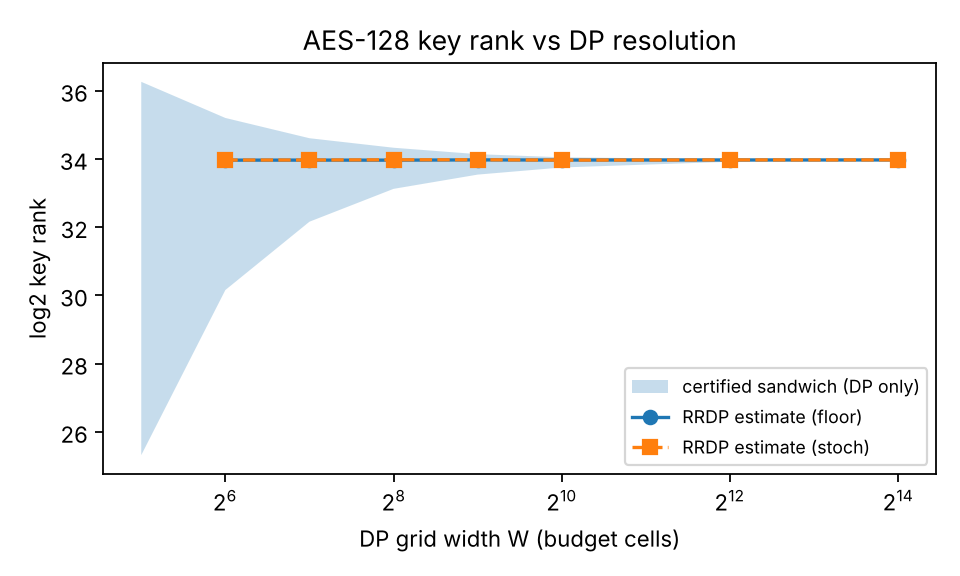
\includegraphics[width=.72\linewidth]{../results/aes_rank.png}
\caption{The deterministic sandwich narrows only as the DP is refined. The randomized correction
is accurate at every resolution where it runs.}\label{fig:aes}
\end{figure}

\paragraph{Floor vs.\ stochastic rounding.} We used synthetic exponential scores, $K=16$, $W=16m$, a partially
leaked key, and $2\cdot10^4$ samples per point.

\begin{table}[h]\centering\small
\resizebox{\linewidth}{!}{\begin{tabular}{@{}rccccc@{}}
\toprule
$m$ & mean floor bias $/D$ ($=m/2$) & stochastic slack $\tau/D$ & acceptance (floor) & acceptance (stoch.) & sample saving \\ \midrule
8 & 4.0 & 4.29 & 0.939 & 0.922 & $0.98\times$ \\
16 & 8.0 & 6.07 & 0.788 & 0.809 & $1.03\times$ \\
32 & 16.0 & 8.58 & 0.614 & 0.776 & $1.26\times$ \\
64 & 32.0 & 12.14 & 0.410 & 0.620 & $1.51\times$ \\
128 & 64.0 & 17.17 & 0.150 & 0.521 & $3.48\times$ \\ \bottomrule
\end{tabular}}
\caption{Stochastic rounding wins once $\sqrt{m\ln(1/\eta)/2}<m/2$, here at about $m\ge16$, as Lemma~\ref{lem:stoch} predicts.}\label{tab:scaling}
\end{table}

\subsection{Findings}
\begin{enumerate}[leftmargin=*]
\item \textbf{RQ1, rounding plus DP.} The DP on a rounded instance yields a certified sandwich whose width is
      governed by $m$ grid cells (Lemma~\ref{lem:sandwich}). It is reliable but biased, and coarse grids give loose bounds
      (10.9 bits at $W=32$).
\item \textbf{RQ2, randomized correction.} Sampling exactly from the rounded DP and rejecting removes the bias
      \emph{completely}: $\E[\hat R]=R$, with $(1\pm\eps)$ accuracy (Theorem~\ref{thm:floor}). A Dyer-type injection bound
      (Lemma~\ref{lem:dyer}) makes this an FPRAS for key rank, which is a \#P-hard problem (Corollary~\ref{cor:fpras}, Proposition~\ref{prop:hard}).
\item \textbf{RQ3, randomized rounding of inputs.} Unbiased shared-shift rounding cuts the error band from $\Theta(mD)$ to
      $O(D\sqrt{m\log(1/\eta)})$ at the cost of a one-sided bias of at most $\eta R$ (Theorem~\ref{thm:stoch}). It pays off for
      many subkeys (up to $3.5\times$ fewer samples at $m=128$) but not for $m\le16$.
\item \textbf{An honest caveat for AES-128.} With $m=16$ the DP is so cheap that a fine grid ($W=16384$) is the fastest
      option overall. Randomized rounding matters when the DP width is the bottleneck: many subkeys (bit-level or
      AES-256 / post-quantum key schedules), multi-constraint DPs, or tight memory such as on-device evaluation.
\end{enumerate}

\noindent In one line: \emph{rounding makes the DP small, the DP makes exact sampling possible, and
sampling makes the rounding error vanish in expectation.}
